%%%%%%%%%%%%%%%%%%%%%%%%%%%%%%%%%%%%%%%%%%%%%%%%%%%%%%%%%%%%%%%%%%%%%%
% LaTeX Template: Beamer arrows
%
% Source: http://www.texample.net/
% Feel free to distribute this template, but please keep the
% referal to TeXample.net.
% Date: Nov 2006
% 
%%%%%%%%%%%%%%%%%%%%%%%%%%%%%%%%%%%%%%%%%%%%%%%%%%%%%%%%%%%%%%%%%%%%%%
% If you're new to LaTeX, the wikibook is a great place to start:
% http://en.wikibooks.org/wiki/LaTeX
%%%%%%%%%%%%%%%%%%%%%%%%%%%%%%%%%%%%%%%%%%%%%%%%%%%%%%%%%%%%%%%%%%%%%%

\documentclass{beamer} %
\usetheme{CambridgeUS}
\usepackage[latin1]{inputenc}
\usefonttheme{professionalfonts}
\usepackage{times}
\usepackage{tikz}
\usepackage{amsmath}
\usepackage{verbatim}
\usepackage{mathtools}
\usepackage{tcolorbox}
\setlength{\fboxsep}{0.5mm}
\usetikzlibrary{arrows,shapes}
\usepackage{array}
\newcolumntype{x}[1]{>{\centering\arraybackslash\hspace{0pt}}p{#1}}

\author[Ilaria Lauzana] {Ilaria Lauzana \newline \\ { \small Supervised by Nadia Figueroa and Jos\'e Medina} \newline {\small Prof. Aude Billard} \newline {\small Learning Algorithms and Systems Laboratory}}
\title[Online Segmentation for Multivariate Data]{Online Segmentation for Multivariate Sequential Data}
\date{June 28, 2016}


% \AtBeginSection[]
% {
%   \begin{frame}<beamer>
%     \frametitle{Outline}
%     \tableofcontents[currentsection,currentsubsection]
%   \end{frame}
% }

\begin{document}

\begin{comment}
:Title: Beamer arrows
:Tags: Remember picture, Beamer, Physics & chemistry, Overlays
:Use page: 3

With PGF/TikZ version 1.09 and later, it is possible to draw paths between nodes across
different pictures. This is a useful feature for presentations with the
Beamer package. In this example I've combined the new PGF/TikZ's overlay feature
with Beamer overlays. Download the PDF version to see the result.

**Note.** This only works with PDFTeX, and you have to run PDFTeX twice.

| Author: Kjell Magne Fauske

\end{comment}


% For every picture that defines or uses external nodes, you'll have to
% apply the 'remember picture' style. To avoid some typing, we'll apply
% the style to all pictures.
\tikzstyle{every picture}+=[remember picture]

% By default all math in TikZ nodes are set in inline mode. Change this to
% displaystyle so that we don't get small fractions.
\everymath{\displaystyle}

\begin{frame}
  \titlepage
\end{frame}

\begin{frame}{Outline}
  \tableofcontents
\end{frame}

\section{Introduction to Segmentation and Changepoint Detection}

\begin{frame}
\frametitle{Problem Statement and Motivation}
\begin{figure}
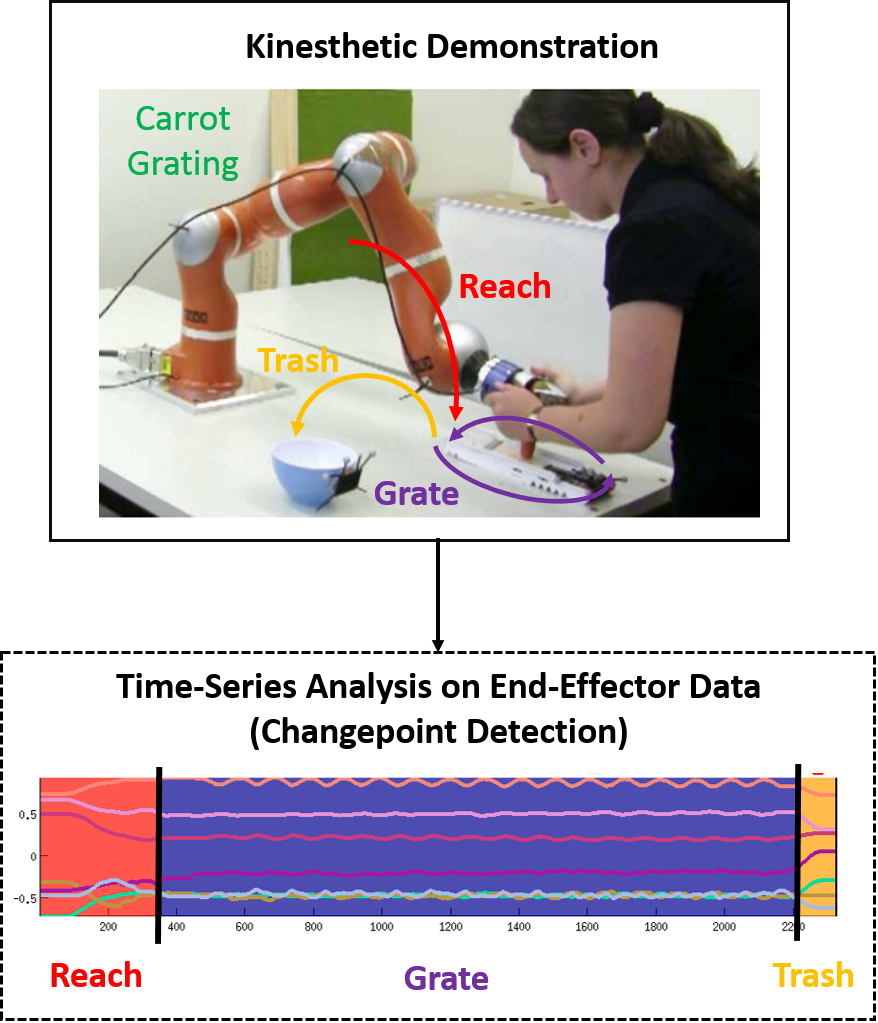
\includegraphics[width=.5\textwidth]{changepoint.png}
%\caption{\label{fig:your-figure}Caption goes here.}
\end{figure}
\end{frame}


\begin{frame}
\frametitle{What is a Changepoint?}
\begin{figure}
\centering
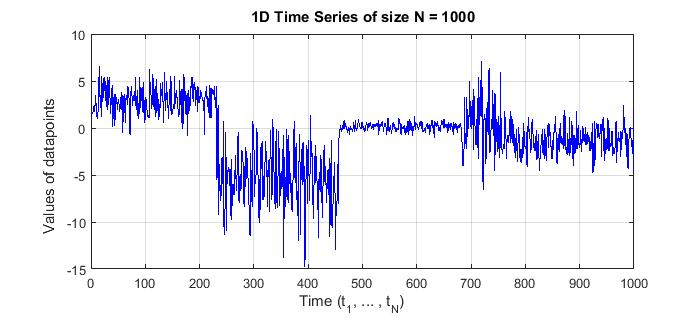
\includegraphics[width=12cm]{1d_series_1000.jpg}
%\caption{\label{fig:your-figure}Caption goes here.}
\end{figure}
\end{frame}


\begin{frame}
\frametitle{What is a Changepoint?}
\begin{figure}
\centering
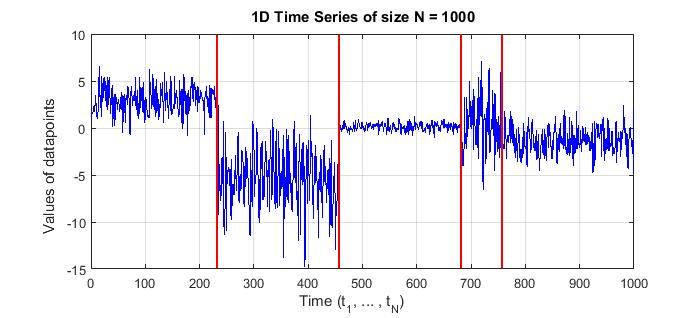
\includegraphics[width=12cm]{1d_series_1000_segments.jpg}
%\caption{\label{fig:your-figure}Caption goes here.}
\end{figure}
\end{frame}


\begin{frame}
\frametitle{Literature Review}
\let\thefootnote\relax\footnote{\color{red}[1] Adams, MacKay (2007), Bayesian Online Changepoint Detection}
\footnotetext{[2] Fearnhead (2006), Exact and efficient Bayesian inference for multiple changepoint problems}
\footnotetext{[3] Niekum, et al. (2014), CHAMP: Changepoint Detection Using Approximate Model Parameters}

\begin{minipage}{.49\textwidth}
\visible<1->{\begin{tcolorbox}[colback=yellow]
Bayesian: \\
\fcolorbox{black}{lime}{Prior on segment length} \\
\fcolorbox{black}{orange}{Prior on model parameters}
\end{tcolorbox}}
\visible<2->{\begin{tcolorbox}[colback=red]
Only for Univariate
\end{tcolorbox}}
\end{minipage}%
\begin{minipage}{.05\textwidth}
\end{minipage}
\begin{minipage}{.49\textwidth}
\visible<3->{\begin{tcolorbox}[colback=green]
\textbf{Proposed Approach:} \\
Extend Adams, MacKay (2007) to Multivariate
\end{tcolorbox}}
\end{minipage}


\end{frame}


\section{Univariate Bayesian Changepoint Detection}

\begin{frame}
\frametitle{Univariate Bayesian Changepoint Detection}
\begin{itemize}
\item Algorithm by Adams and MacKay: finds posterior probability of "run length" $r_t$ (= time since the last changepoint); is online
% \item Inference can be performed online as probabilities are updated after each new sample
\item \fcolorbox{black}{lime}{Uniform prior on segment length}:
\[\pi(r_t) = P(r_t | r_{t - 1}) = 1 / \lambda\]
\item \fcolorbox{black}{orange}{
Conjugate prior on model parameters} for 1D Gaussian with unknown mean $\mu$ and unknown variance $\sigma^2$:
\[ \pi(\mu,\sigma^2) = NIG(\mu, \sigma^2 | \mu_0, \kappa_0, \alpha_0, \beta_0)\]
% \begin{figure}
% 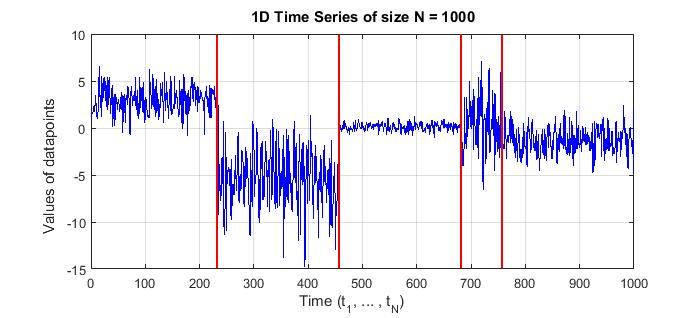
\includegraphics[width=11cm]{1d_series_1000_segments.jpg}
% %\caption{\label{fig:your-figure}Caption goes here.}
% \end{figure}
\end{itemize}
\end{frame}


% \begin{frame}
% \frametitle{Prior on model parameters}
% \begin{itemize}
% \item To find the posterior predictive distribution for new observation $\tilde{x}$: \[ P(\tilde{x} | X, \eta) = \int P(\tilde{x} | \theta) P(\theta | X, \eta) d\theta, \] where $\pi(\theta) = P(\theta | X, \eta)$ is the prior on the model parameters $\theta$, with parameters $\eta$
% \item Predictive posterior represents likelihood of data given the computed model parameters
% \item Use a $conjugate$ $prior$ for the model of data:
% \begin{itemize}
% \item obtain a posterior distribution in the same form of the prior
% \item avoid the integration and obtain posterior's parameters $\eta_n$ from the prior's parameters $\eta$ and from the sampled data
% \end{itemize}
% \end{itemize}
% \end{frame}

% \begin{frame}
% \frametitle{Prior on model parameters}
% \begin{itemize}
% \item 1D Gaussian with unknown mean $\mu$ and unknown variance $\sigma^2$
% \item Conjugate prior to the model is a Normal-Inverse-Gamma  distribution with parameters \(\eta_0 =  (\mu_0, \kappa_0, \alpha_0, \beta_0)\): \[ \pi(\mu,\sigma^2) = NIG(\mu, \sigma^2 | \mu_0, \kappa_0, \alpha_0, \beta_0),\]%= N(\mu | \mu_0, \kappa_0\sigma^2)\Gamma^{-1}(\sigma^2 | \alpha_0, \beta_0)\
% \item Posterior predictive distribution is also NIG and its parameters \(\eta_n =  (\mu_n, \kappa_n, \alpha_n, \beta_n)\):
% \[\mu_n = \frac{\kappa_0\mu_0 + n\bar{x}}{\kappa_0 + n}, \]
% \[\kappa_n = \kappa_0 + n,\]
% \[\alpha_n = \alpha_0 + n/2,\]
% \[\beta_n = \beta_0 + \frac{1}{2} \sum_{i=1}^{n} (x_i - \bar{x})^2 + \frac{\kappa_0n(\bar{x} - \mu_0)^2}{2(\kappa_0 + n)}. \] 
% \end{itemize}
% \end{frame}



\begin{frame}
\frametitle{Algorithm}
% The algorithm used tries to find the value the current run length $r_t$ by reusing previous inference results in the calculation of the current time's posterior distribution.
\begin{itemize}
\visible<1->{\item \fcolorbox{black}{orange}{Initialize parameters \(\eta_0 = (\mu_0, \kappa_0, \alpha_0, \beta_0)\) of the NIG prior}
\item Iterate for $t$ up to $N$:}
\begin{enumerate}
\visible<2->{\item Predictive posterior distribution of the new observation $x_t$: \\ \begin{center}
\fcolorbox{black}{orange}{ $P (x_t | x_{1:t-1}, \eta_t) = NIG(\eta_t = (\mu_t, \kappa_t, \alpha_t, \beta_t))$}
\end{center}}
\vspace{0.2cm}
\visible<3->{\item Joint probabilities for each run length $r_t$: \[ \underbrace{P(r_t , x_{1:t})}_{\text{\shortstack{Joint distribution \\ at current time step}}} = \underbrace{P(r_{t-1} , x_{1:(t-1)})}_{\text{\shortstack{Joint distribution \\ at previous time step}}}  \underbrace{\fcolorbox{black}{orange}{ $P (x_t | x_{1:t-1}, \eta_t)$}}_{\text{\shortstack{Predictive distribution \\ of new observation}}}  \underbrace{\fcolorbox{black}{lime}{$P(r_t | r_{t - 1})$}}_{\text{\shortstack{Prior on \\ segment length}}}\]}
\visible<4->{\item Posterior probabilities: \[ P(r_t | x_{1:t}) = \frac{P(r_t , x_{1:t})}{\sum_{j=0}^{t} P(r_t = j , x_{1:t}) }\]}
\visible<5->{\item \fcolorbox{black}{orange}{Update parameters $\eta_t$}}
\end{enumerate}
\end{itemize}
\end{frame}


\begin{frame}
\frametitle{1D Gaussian distribution with noise}
\begin{itemize}
\item On top: time series, changepoints in red
\item On bottom: posterior probabilities for each run length, max posterior in red
\end{itemize}
\begin{figure}
\centering
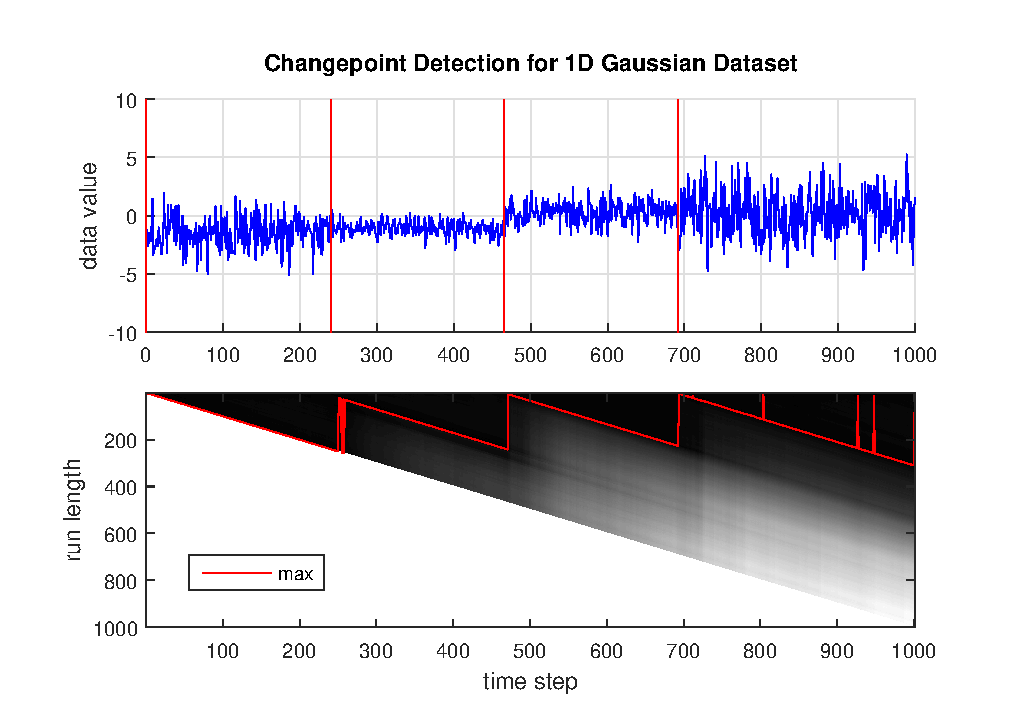
\includegraphics[width=.7\linewidth]{1d_gauss.eps}
\end{figure}
\end{frame}


\section{Multivariate Bayesian Changepoint Detection}


\begin{frame}
\frametitle{From univariate to multivariate data}
\begin{itemize}
\item Data is sampled from a Multivariate Gaussian $N(\boldsymbol{\mu}, \boldsymbol{\Sigma})$
\item The conjugate prior to the model is a Normal-Inverse-Wishart (NIW) distribution \[NIW(\boldsymbol{\mu}, \boldsymbol{\Sigma} | \underbrace{\boldsymbol{\mu_0}}_{\text{Mean}}, \underbrace{\kappa_0}_{\text{\shortstack{Scaling \\ factor}}}, \underbrace{\nu_0}_{\text{\shortstack{Degrees of \\ freedom}}}, \underbrace{\boldsymbol{\Lambda_0}}_{\text{\shortstack{Inverse \\ scale matrix}}})\]
\item The posterior predictive is a NIW distribution with parameters:
\[\boldsymbol{\mu_n} = \frac{\kappa_0\boldsymbol{\mu_0} + n\boldsymbol{\bar{x}}}{\kappa_0 + n}, \]
\[\kappa_n = \kappa_0 + n,\]
\[\nu_n = \nu_0 + n,\]
\[\boldsymbol{\Lambda_n} = \boldsymbol{\Lambda_0} + \boldsymbol{S} + \frac{\kappa_0n}{\kappa_0 + n}(\boldsymbol{\bar{x}} - \boldsymbol{\mu_0})(\boldsymbol{\bar{x}} - \boldsymbol{\mu_0})^T, \]
\centering S is the scatter matrix: \(\boldsymbol{S} = \sum(\boldsymbol{x_i} - \boldsymbol{\bar{x}})(\boldsymbol{x_i} - \boldsymbol{\bar{x}})^T\)
\end{itemize}
\end{frame}


\begin{frame}
\frametitle{From univariate to multivariate data}
\centering
\hspace{\dimexpr-\fboxrule-\fboxsep\relax}\fbox{\begin{minipage}{0.45\textwidth}
\begin{itemize}
\item \textcolor{red}{Initialize parameters \(\eta_0 = (\mu_0, \kappa_0, \alpha_0, \beta_0)\) of the NIG prior}
\item Iterate for $t$ up to $N$:
\begin{enumerate}
\item \textcolor{red}{Predictive distribution: \( P (x_t | x_{1:t-1}, \eta_t) = \) \(NIG(\mu_t, \kappa_t, \alpha_t, \beta_t)\)}
\item Joint probabilities: \[P(r_t , x_{1:t})\]
\item Posterior probabilities: \[ P(r_t | x_{1:t}) \]
\item \textcolor{red}{Update parameters $\eta_t$ }
\end{enumerate}
\end{itemize}
\end{minipage}
}
\begin{minipage}{0.01\textwidth}
\end{minipage}
\hspace{\dimexpr-\fboxrule-\fboxsep\relax}\fbox{\begin{minipage}{0.45\textwidth}
\begin{itemize}
\item \textcolor{red}{Initialize parameters \(\eta_0 = (\boldsymbol{\mu_0}, \kappa_0, \nu_0, \boldsymbol{\Lambda_0})\) of the NIW prior}
\item Iterate for $t$ up to $N$:
\begin{enumerate}
\item \textcolor{red}{Predictive distribution: \( P (\boldsymbol{x_t} | \boldsymbol{x_{1:t-1}}, \eta_t) =\) \(NIW(\boldsymbol{\mu_t}, \kappa_t, \nu_t, \boldsymbol{\Lambda_t})\)}
\item Joint probabilities: \[P(r_t , \boldsymbol{x_{1:t}})\]
\item Posterior probabilities: \[ P(r_t | \boldsymbol{x_{1:t}}) \]
\item \textcolor{red}{Update parameters $\eta_t$ }
\end{enumerate}
\end{itemize}
\end{minipage}
}
\end{frame}


\begin{frame}
\frametitle{6D Gaussian distribution with noise}
\begin{figure}
\centering
% \begin{minipage}{.5\textwidth}
  %\centering
  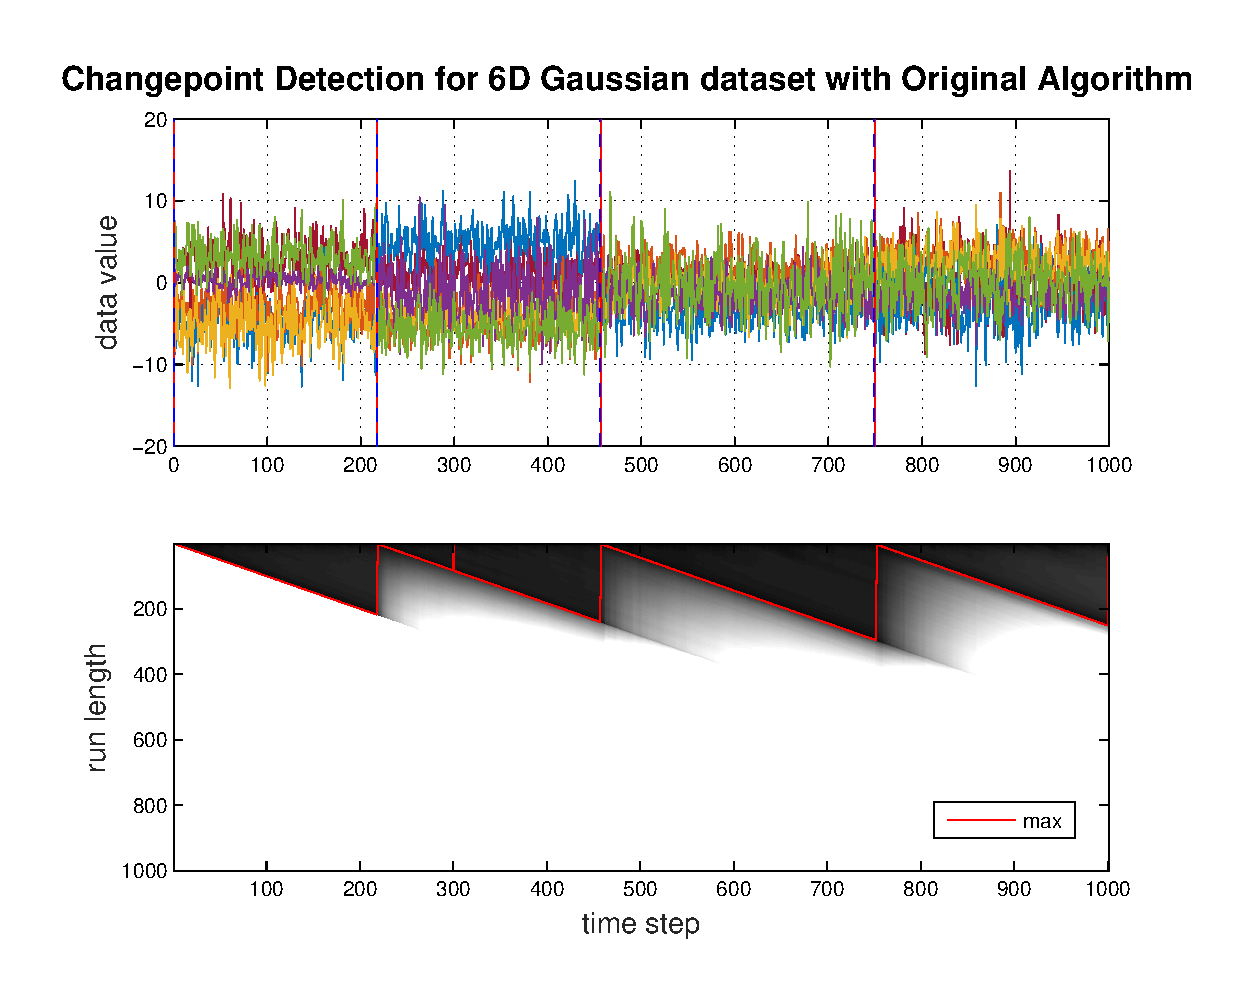
\includegraphics[height=.85\textheight]{6d_gauss_full.eps}
% \end{minipage}%
% \begin{minipage}{.5\textwidth}
%   %centering
%   \includegraphics[width=\linewidth]{2d_toy_fast.jpg}
% \end{minipage}
\end{figure}
\end{frame}


\begin{frame}
\frametitle{Limitations}
\begin{itemize}
\item Increases linearly in complexity with time
% computationally intensive $\rightarrow$ need to compute $t$ times the predictive, joint and posterior probabilities (for all possible $r_t$ at each time step $t$)
\vspace{1cm}
\item \textbf{Proposal}: \textit{truncated} version, considering only run lengths values feasible since the last changepoint
\end{itemize}
\end{frame}

\begin{frame}
\frametitle{Truncated Multivariate Algorithm}
\begin{itemize}
\item Initialize parameters \(\eta_0 = (\boldsymbol{\mu_0}, \kappa_0, \nu_0, \boldsymbol{\Lambda_0})\) of the NIW prior
\item Iterate for $t$ up to $N$:
\begin{enumerate}
\item Predictive distribution: \[P (\boldsymbol{x_t} | \boldsymbol{x_{1:t-1}}, \eta_t) = NIW(\eta_t = (\boldsymbol{\mu_t}, \kappa_t, \nu_t, \boldsymbol{\Lambda_t}))\]
\item Joint probabilities: \[P(r_t , \boldsymbol{x_{1:t}})\]
\item Posterior probabilities: \[ P(r_t | \boldsymbol{x_{1:t}}) \]
\item \textcolor{blue}{ Current run length: \[r_t = arg\max( P(r_t | \boldsymbol{x_{1:t}}) )\]
\item If \(r_t < r_{t-1} \) $\rightarrow$ store: changepoint $lastCP = t -r_t$, parameters $\eta_{t-r_t}$}
\item Update parameters $\eta_t$ \textcolor{blue}{considering only data from $lastCP$ to $t$} 
\end{enumerate}
\end{itemize}
\end{frame}

% \begin{frame}
% \frametitle{Experiments setup}
% \begin{itemize}
% \item Experiments are run offline but iterating over the whole time series to simulate online behaviour
% \item Both data generated by prior distributions and real datasets
% \item For each time step $t$, the algorithm finds the run length $r_t$ with higher probability. Changepoints located at $t - r_t$ and may be found during run time by checking evolution of run length
% \item Original algorithm computes predictive and joint probabilities for all possible run lengths at each time step, with time growing linearly with the number of datapoints
% \item An additional "fast" version of the algorithm was implemented to cut the time by considering only run lengths values feasible since the last changepoint
% \end{itemize}
% \end{frame}


\section{Results from Experiments}

% \begin{frame}
% \frametitle{6D Gaussian distribution with noise and fast algorithm}
% \begin{figure}
% \centering
% 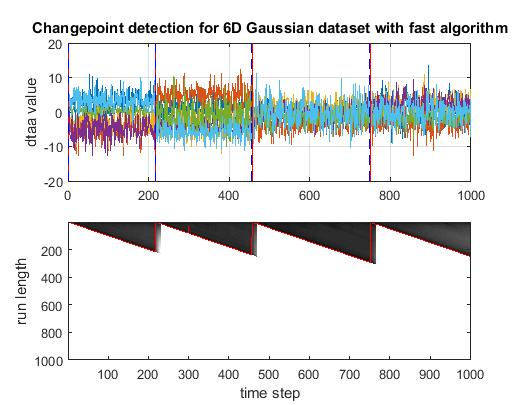
\includegraphics[height=.8\textheight]{6d_gauss_fast.jpg}
% \end{figure}
% \end{frame}

\begin{frame}
\frametitle{6D Gaussian distribution with noise: original and truncated}
\begin{figure}
\centering
\begin{minipage}{.5\textwidth}
  \centering
  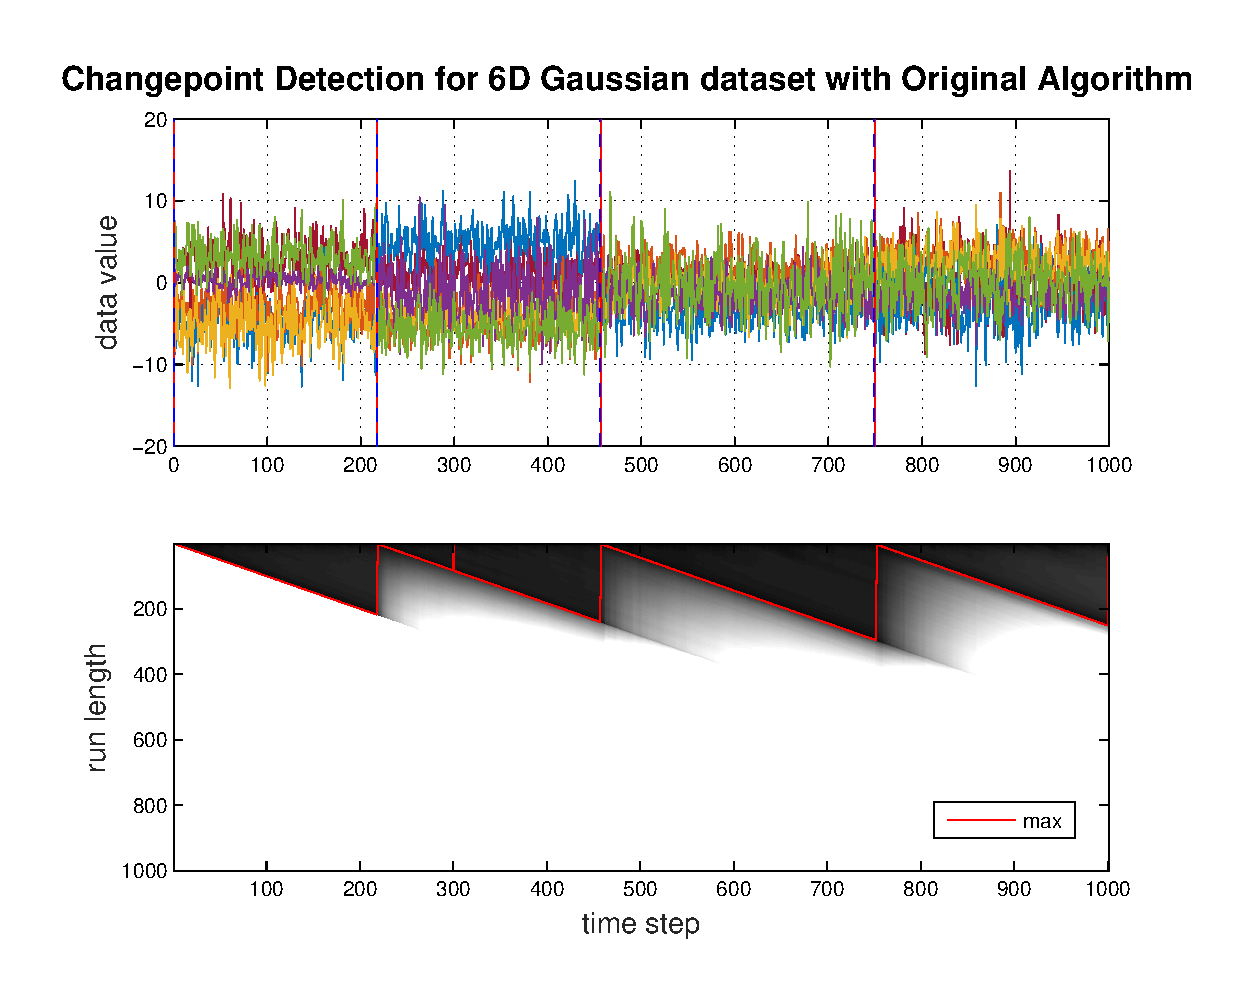
\includegraphics[width=\linewidth]{6d_gauss_full.eps}
\end{minipage}%
\begin{minipage}{.5\textwidth}
  \centering
  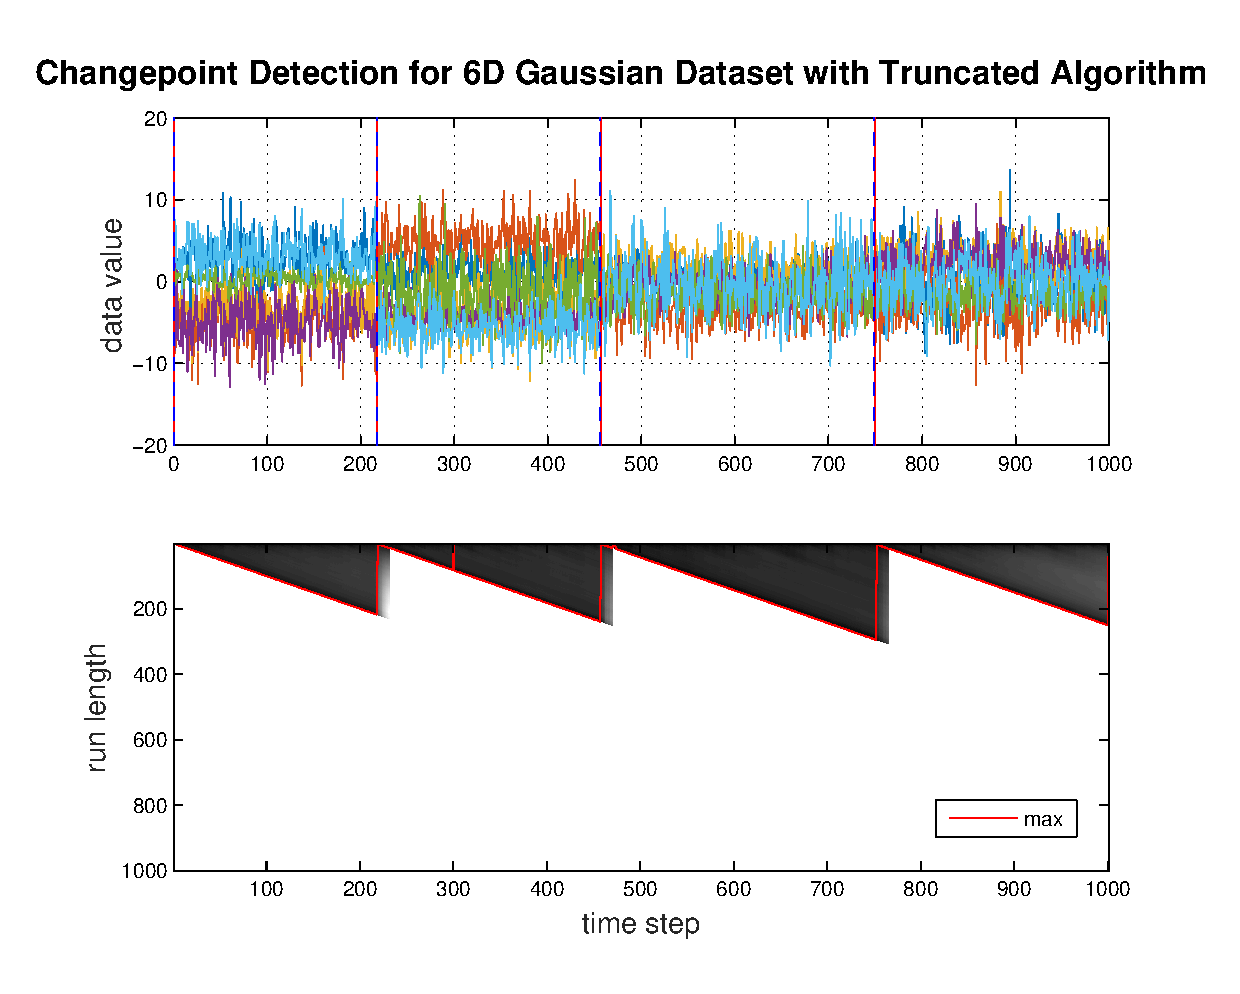
\includegraphics[width=\textwidth]{6d_gauss_fast.eps}
\end{minipage}
\end{figure}
\end{frame}

\begin{frame}
\frametitle{Computation time for detection for 6D Gaussian: original and truncated}
\vfill
\begin{tabular}{|x{2.7cm}|x{4cm}|x{4cm}|}
\hline
\textbf{Changepoint Location} & \textbf{Time of Detection (s) Original Algorithm} & \textbf{Time of Detection (s) Truncated Algorithm} \\ \hline
0 & 0 & 0 \\ \hline
217 & 0.7880 & 0.6063 \\ \hline
456 & 1.3382 & 0.5193 \\ \hline
749 & 1.6176 & 0.6144 \\ \hline
\end{tabular}
\vfill
\begin{itemize}
\item Time from real changepoint occurrence to detection by algorithm
\item Changepoint at 0 known a priori $\rightarrow$ 0 s for detection
\end{itemize}
\end{frame}

\begin{frame}
\frametitle{Time comparison for 2-10 dimensions}
\begin{figure}
\centering
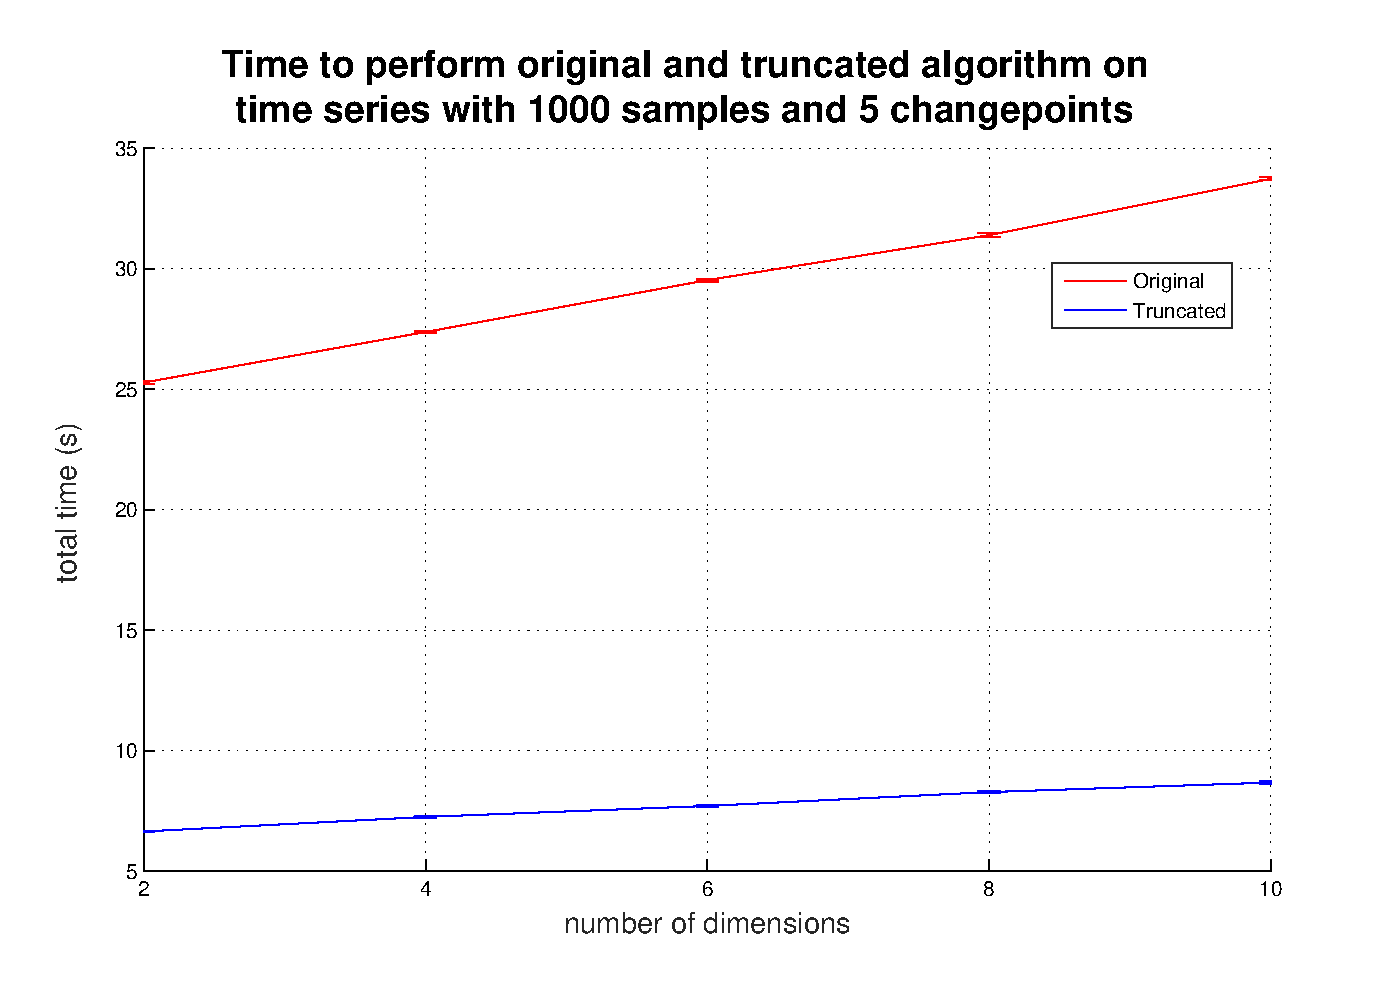
\includegraphics[height=.85\textheight]{plot_time.eps}
\end{figure}
\end{frame}


\begin{frame}
\frametitle{7D real dataset of Carrot Grating task}
\begin{itemize}
\item Real dataset, 7 dimensions: $x$, $y$, $z$ and quaternions $q_i$, $q_j$, $q_k$, $q_w$
\end{itemize}
\begin{figure}
\centering
\begin{minipage}{.5\textwidth}
  \centering
  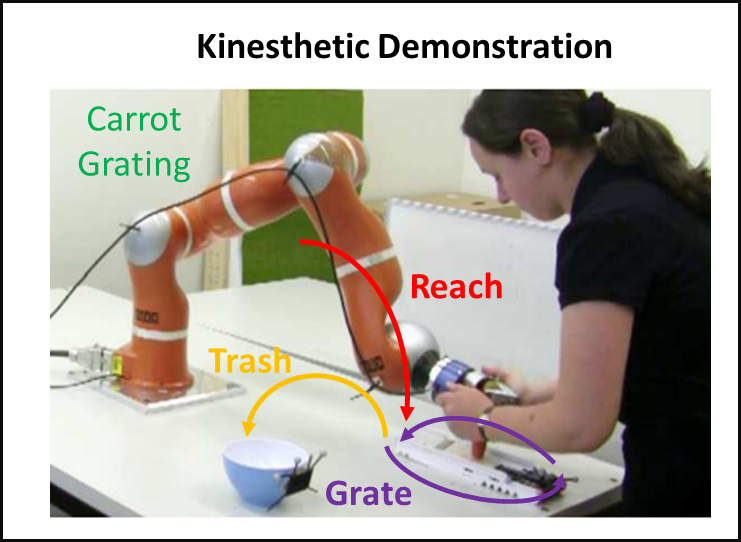
\includegraphics[width=.9\linewidth]{carrot_grating.png}
\end{minipage}%
\begin{minipage}{.5\textwidth}
  %\centering
  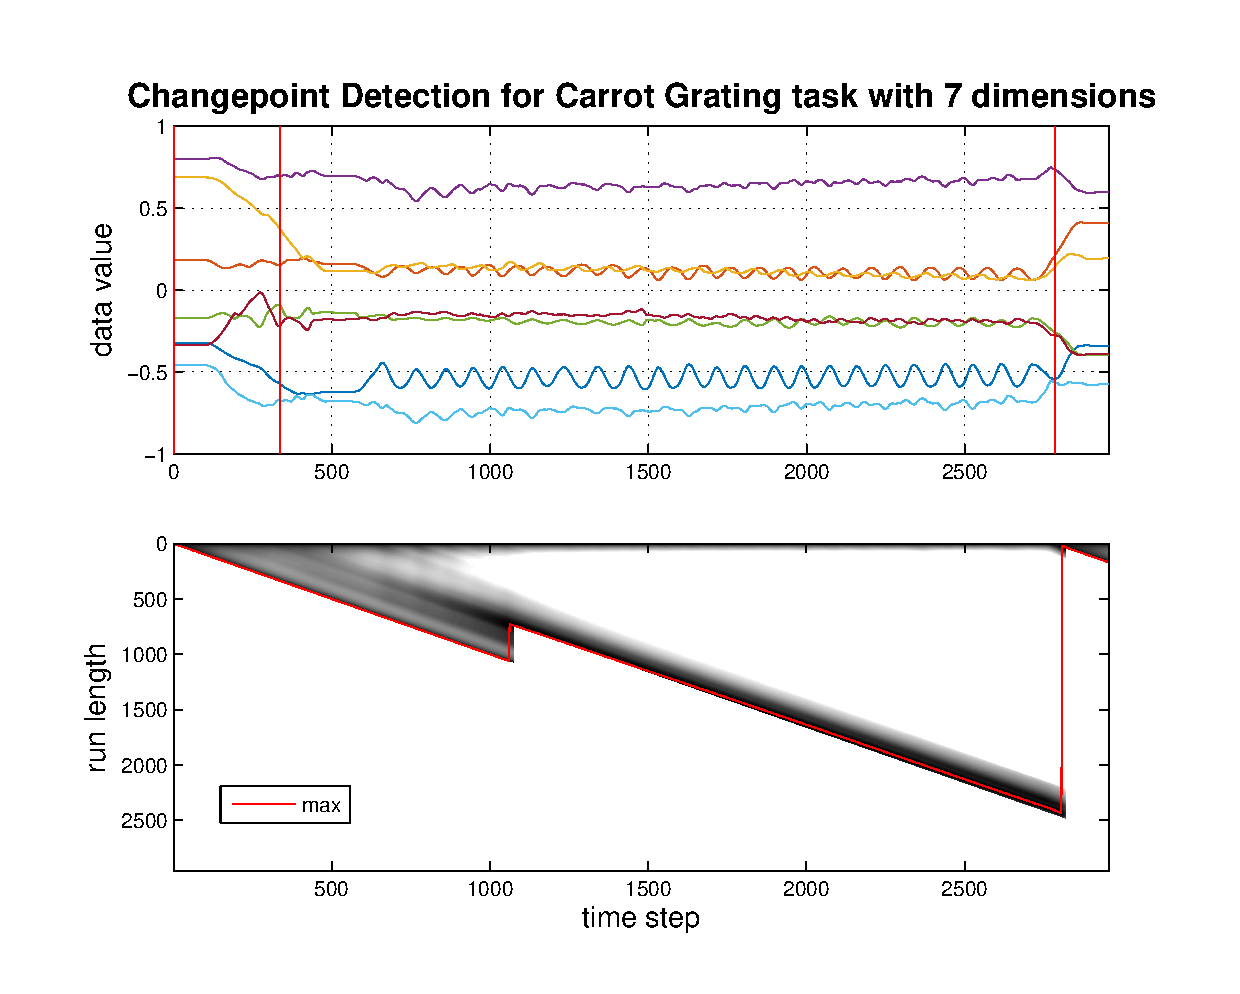
\includegraphics[width=\linewidth]{carrot_fast.eps}
\end{minipage}
\end{figure}
\end{frame}

\begin{frame}
\frametitle{7D real dataset of Zucchini Peeling task}
\begin{itemize}
\item Real dataset, 7 dimensions: $x$, $y$, $z$ and quaternions $q_i$, $q_j$, $q_k$, $q_w$
\end{itemize}
\begin{figure}
\centering
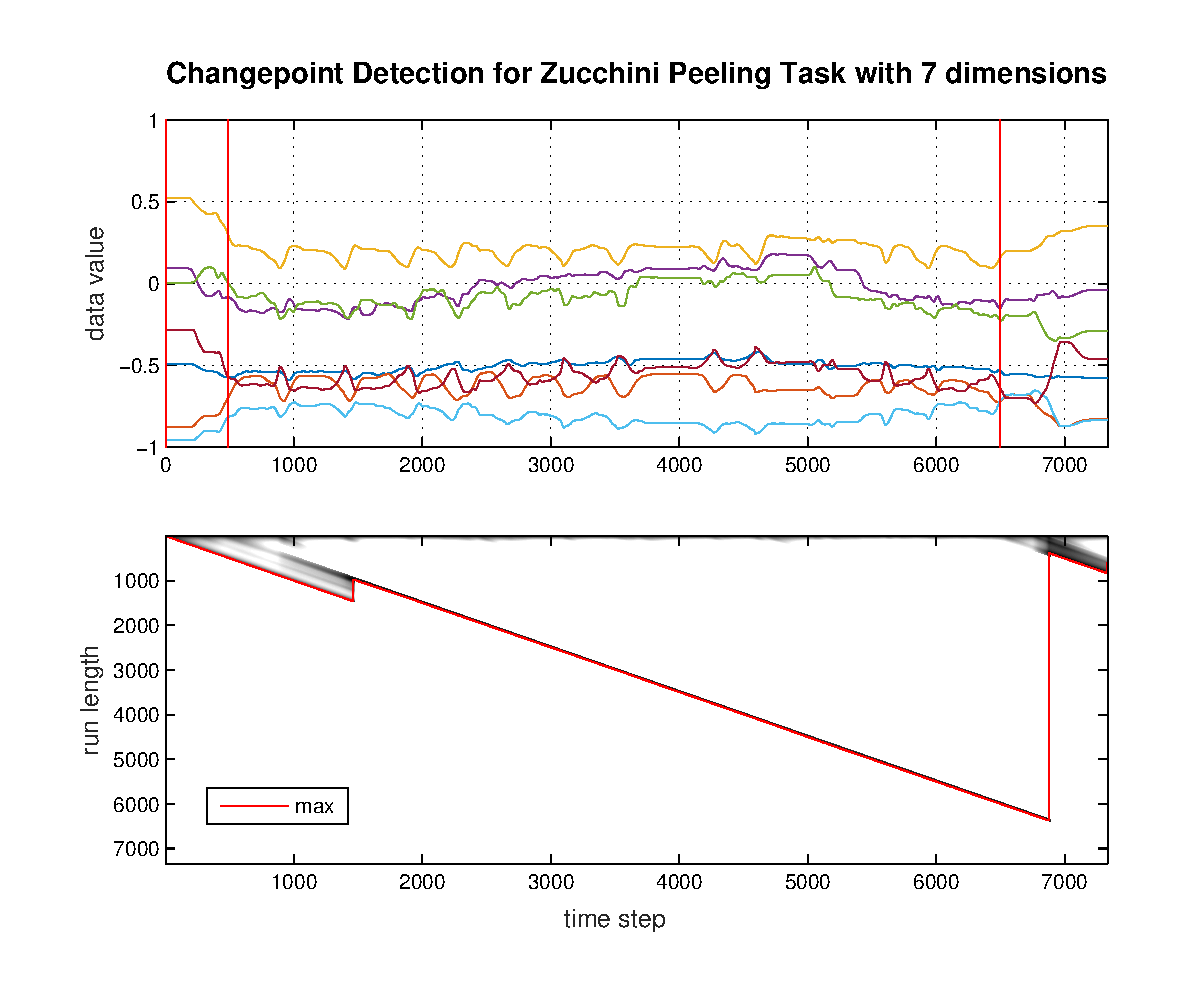
\includegraphics[height=.8\textheight]{proc2_7dim.eps}
\end{figure}
\vfill
\end{frame}

\begin{frame}
\frametitle{13D real dataset of Zucchini Peeling task}
\begin{itemize}
\item First 7 dimensions: $x$, $y$, $z$ and quaternions $q_i$, $q_j$, $q_k$, $q_w$
\item Additional 6 dimensions: forces and torques on end effector
\end{itemize}
\begin{figure}
\centering
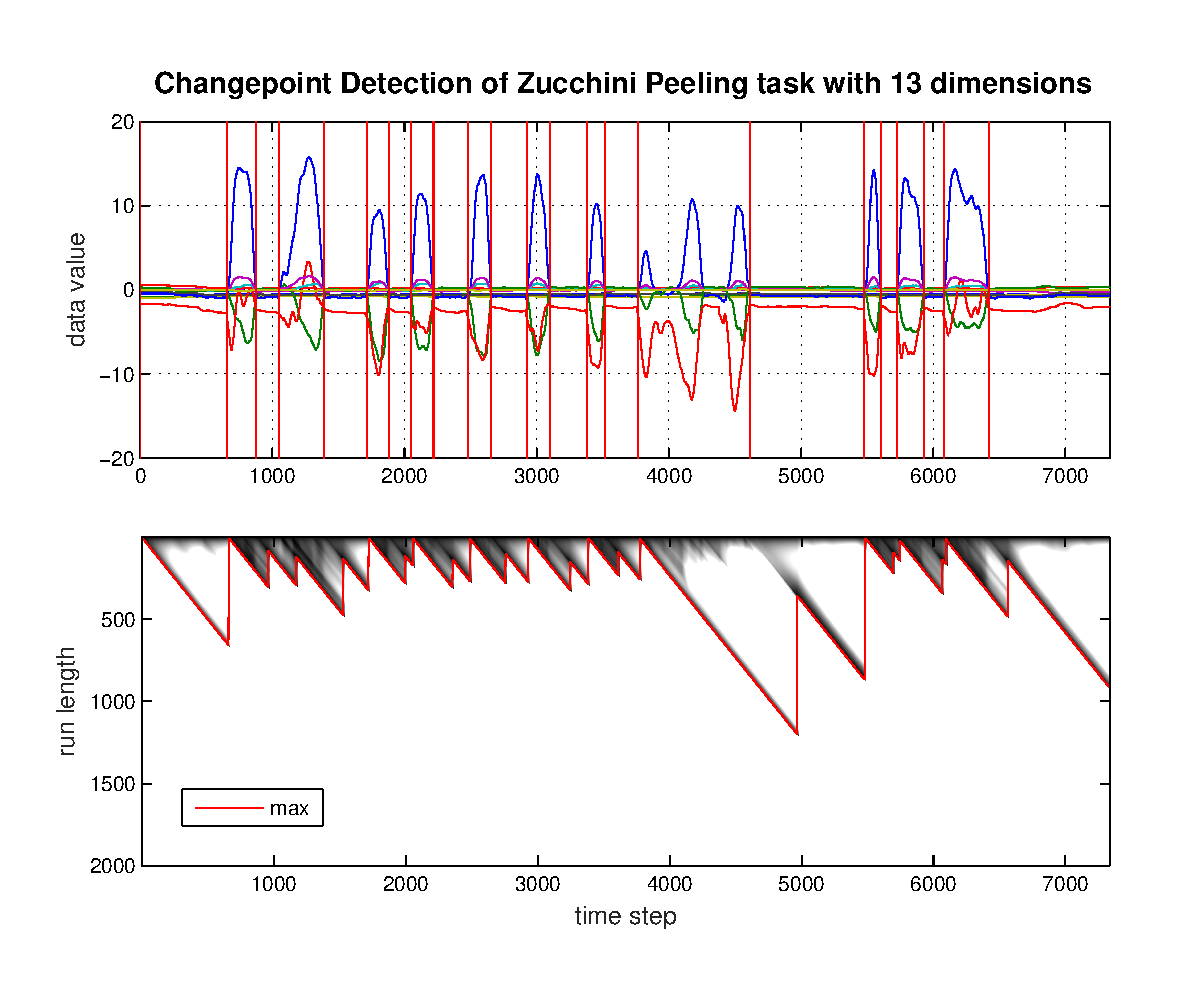
\includegraphics[height=.76\textheight]{proc2.eps}
\end{figure}
\end{frame}



\section{Conclusion}

\begin{frame}
\frametitle{Conclusion}
\begin{itemize}
% \item Perform new simulations on real datasets, with higher number of dimensions and number of datapoints
% \item Explore different priors on segment length
% \item Implement algorithm as a ROS node to test it in real time with robot data
\item Online Segmentation Algorithm for Multivariate Data, implemented in MATLAB, Python and as ROS Node
\item Satisfactory results, comparable to offline batch algorithms on same real datasets
% \item Generally higher level of segmentation $\rightarrow$ pre-process data for learning algorithms
\item \textit{Future steps:}
\begin{itemize}
\item Further experiments on real-time implementation
\item Exploring different priors on segment length
\item Sparsifying computation for algorithm 
\end{itemize}
\end{itemize}
\end{frame}

\begin{frame}
\centering
\huge{Thank you for your attention!}
\end{frame}


% \begin{frame}
% \frametitle{}
% \tikzstyle{na} = [baseline=-.5ex]

% \begin{itemize}[<+-| alert@+>]
%     \item Coriolis acceleration
%         \tikz[na] \node[coordinate] (n1) {};
% \end{itemize}

% Below we mix an ordinary equation with TikZ nodes. Note that we have to
% adjust the baseline of the nodes to get proper alignment with the rest of
% the equation.
% \begin{equation*}
% \vec{a}_p = \vec{a}_o+\frac{{}^bd^2}{dt^2}\vec{r} +
%         \tikz[baseline]{
%             \node[fill=blue!20,anchor=base] (t1)
%             {$ 2\vec{\omega}_{ib}\times\frac{{}^bd}{dt}\vec{r}$};
%         } +
%         \tikz[baseline]{
%             \node[fill=red!20, ellipse,anchor=base] (t2)
%             {$\vec{\alpha}_{ib}\times\vec{r}$};
%         } +
%         \tikz[baseline]{
%             \node[fill=green!20,anchor=base] (t3)
%             {$\vec{\omega}_{ib}\times(\vec{\omega}_{ib}\times\vec{r})$};
%         }
% \end{equation*}

% \begin{itemize}[<+-| alert@+>]
%     \item Transversal acceleration
%         \tikz[na]\node [coordinate] (n2) {};
%     \item Centripetal acceleration
%         \tikz[na]\node [coordinate] (n3) {};
% \end{itemize}

% Now it's time to draw some edges between the global nodes. Note that we
% have to apply the 'overlay' style.
% \begin{tikzpicture}[overlay]
%         \path[->]<1-> (n1) edge [bend left] (t1);
%         \path[->]<2-> (n2) edge [bend right] (t2);
%         \path[->]<3-> (n3) edge [out=0, in=-90] (t3);
% \end{tikzpicture}
% \end{frame}

\end{document}